\documentclass[tikz,border=3pt]{standalone}
\usepackage[T1]{fontenc}
\usepackage{helvet}
\renewcommand{\familydefault}{\sfdefault}
\usetikzlibrary{arrows.meta,positioning,fit,backgrounds}
\definecolor{ink}{HTML}{17324B}
\definecolor{attack}{HTML}{AA3377}
\definecolor{pale}{HTML}{F0F5F8}
\begin{document}
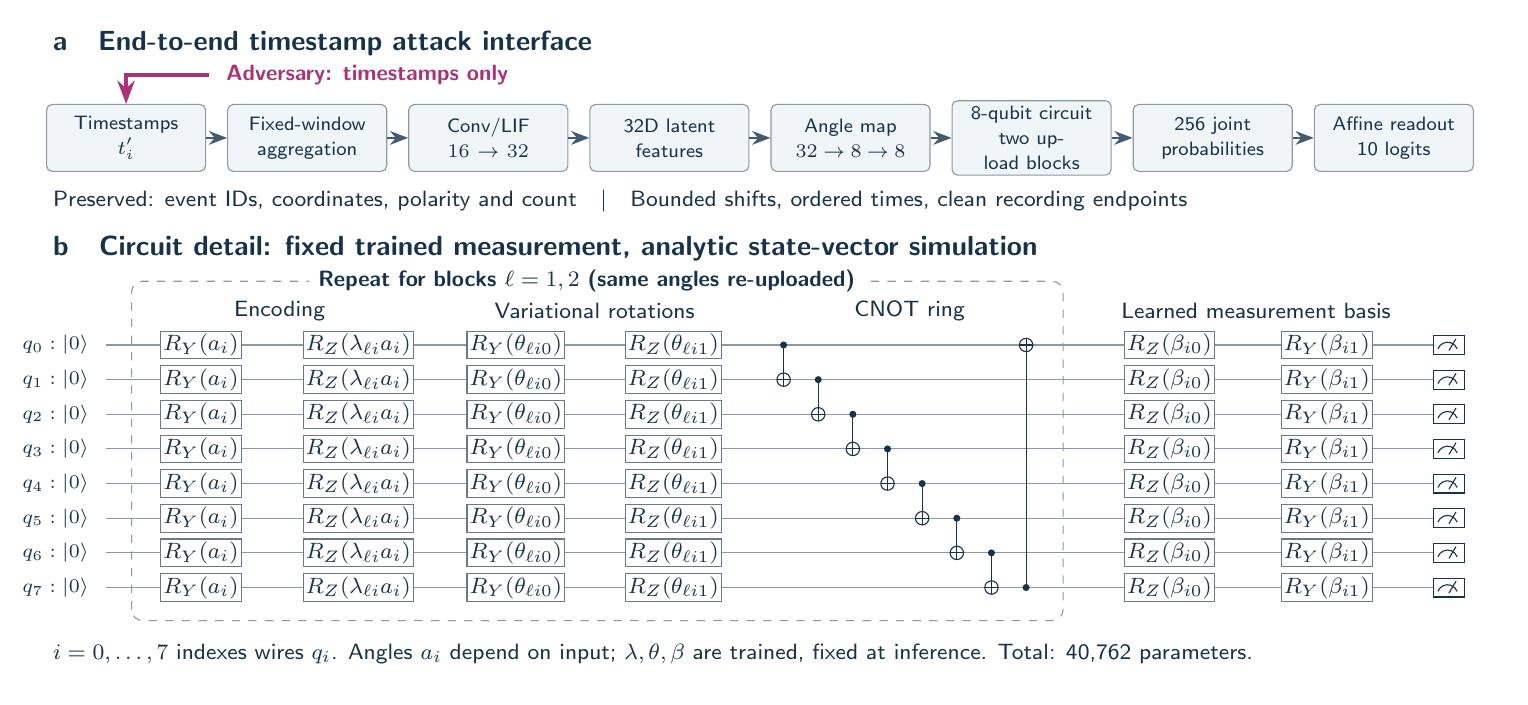
\begin{tikzpicture}[x=1cm,y=1cm, text=ink, >=Stealth,
 stage/.style={draw=ink!50,fill=pale,rounded corners=2pt,text width=1.87cm,minimum width=2.02cm,minimum height=.85cm,inner sep=2pt,align=center,font=\fontsize{7.5}{9}\selectfont},
 gate/.style={draw=ink!65,fill=white,minimum width=.95cm,minimum height=.31cm,inner sep=1pt,font=\fontsize{8}{9}\selectfont}]
\path[use as bounding box](-.2,-.1) rectangle(18.5,8.15);
\node[anchor=west,font=\bfseries\fontsize{10}{12}\selectfont] at(0,7.95){a\quad End-to-end timestamp attack interface};
\foreach \x/\name/\label in {1.05/t/{Timestamps\\$t'_i$},3.35/ag/{Fixed-window\\aggregation},5.65/lif/{Conv/LIF\\$16\!\to\!32$},7.95/latent/{32D latent\\features},10.25/angle/{Angle map\\$32\!\to\!8\!\to\!8$},12.55/q/{8-qubit circuit\\two upload blocks},14.85/prob/{256 joint\\probabilities},17.15/logits/{Affine readout\\10 logits}}
 {\node[stage](\name) at(\x,6.75){\label};}
\foreach \a/\b in {t/ag,ag/lif,lif/latent,latent/angle,angle/q,q/prob,prob/logits}
 {\draw[->,thick,ink!80](\a.east)--(\b.west);}
\node[text=attack,font=\bfseries\fontsize{8}{9}\selectfont,anchor=west] at(2.2,7.55){Adversary: timestamps only};
\draw[->,very thick,attack](2.1,7.55)-|(t.north);
\node[anchor=west,font=\fontsize{8}{10}\selectfont] at(0,5.95){Preserved: event IDs, coordinates, polarity and count\quad\textbar\quad Bounded shifts, ordered times, clean recording endpoints};
\node[anchor=west,font=\bfseries\fontsize{10}{12}\selectfont] at(0,5.35){b\quad Circuit detail: fixed trained measurement, analytic state-vector simulation};
\draw[dashed,ink!50,rounded corners] (1.12,.62) rectangle(12.95,4.93);
\node[fill=white,font=\bfseries\fontsize{8}{10}\selectfont] at(6.9,4.93){Repeat for blocks $\ell=1,2$ (same angles re-uploaded)};
\node[font=\fontsize{8}{10}\selectfont] at(3,4.55){Encoding};
\node[font=\fontsize{8}{10}\selectfont] at(7,4.55){Variational rotations};
\node[font=\fontsize{8}{10}\selectfont] at(11,4.55){CNOT ring};
\node[font=\fontsize{8}{10}\selectfont] at(15.4,4.55){Learned measurement basis};
\foreach \i in {0,...,7}{
 \pgfmathsetmacro{\yy}{4.12-.44*\i}
 \draw[ink!50](.8,\yy)--(17.65,\yy);
 \node[anchor=east,font=\fontsize{7}{8}\selectfont] at(.7,\yy){$q_{\i}:|0\rangle$};
 \node[gate] at(2,\yy){$R_Y(a_i)$};
 \node[gate] at(4,\yy){$R_Z(\lambda_{\ell i}a_i)$};
 \node[gate] at(6,\yy){$R_Y(\theta_{\ell i0})$};
 \node[gate] at(8,\yy){$R_Z(\theta_{\ell i1})$};
 \node[gate] at(14.3,\yy){$R_Z(\beta_{i0})$};
 \node[gate] at(16.3,\yy){$R_Y(\beta_{i1})$};
 \draw[fill=white,draw=ink](17.65,\yy-.12) rectangle(18.05,\yy+.12);
 \draw[ink](17.71,\yy-.05) arc[start angle=160,end angle=20,radius=.13];
 \draw[ink](17.85,\yy-.07)--(17.94,\yy+.08);
}
\foreach \i in {0,...,7}{
 \pgfmathtruncatemacro{\j}{mod(\i+1,8)}
 \pgfmathsetmacro{\xx}{9.4+.44*\i}
 \pgfmathsetmacro{\yc}{4.12-.44*\i}
 \pgfmathsetmacro{\yt}{4.12-.44*\j}
 \draw[ink](\xx,\yc)--(\xx,\yt);
 \fill[ink](\xx,\yc) circle(.045);
 \draw[fill=white,draw=ink](\xx,\yt) circle(.085);
 \draw[ink](\xx-.085,\yt)--(\xx+.085,\yt);
 \draw[ink](\xx,\yt-.085)--(\xx,\yt+.085);
}
\node[anchor=west,font=\fontsize{8}{9}\selectfont] at(0,.2){$i=0,\ldots,7$ indexes wires $q_i$. Angles $a_i$ depend on input; $\lambda,\theta,\beta$ are trained, fixed at inference. Total: 40,762 parameters.};
\end{tikzpicture}
\end{document}
